

% Lecture Template for ME3023-001- Tristan Hill - Spring 2018 - Summer 2018
% 
% Measurements in Mechanical Systems

% Document settings
\documentclass[11pt]{article}
% \usepackage[margin=1in]{geometry}
\usepackage[left=1.5cm, right=1.5cm, top=2cm]{geometry}
\usepackage[pdftex]{graphicx}
\usepackage{multirow}
\usepackage{setspace}
\usepackage{hyperref}
\usepackage{color,soul}
\usepackage{fancyvrb}
\usepackage{framed}
\usepackage{wasysym}
\usepackage{multicol}

\usepackage[utf8]{inputenc}
\usepackage[english]{babel}
 


\pagestyle{plain}
\setlength\parindent{0pt}
\hypersetup{
    bookmarks=true,         % show bookmarks bar?
    unicode=false,          % non-Latin characters in Acrobat’s bookmarks
    pdftoolbar=true,        % show Acrobat’s toolbar?
    pdfmenubar=true,        % show Acrobat’s menu?
    pdffitwindow=false,     % window fit to page when opened
    pdfstartview={FitH},    % fits the width of the page to the window
    pdftitle={My title},    % title
    pdfauthor={Author},     % author
    pdfsubject={Subject},   % subject of the document
    pdfcreator={Creator},   % creator of the document
    pdfproducer={Producer}, % producer of the document
    pdfkeywords={keyword1} {key2} {key3}, % list of keywords
    pdfnewwindow=true,      % links in new window
    colorlinks=true,       % false: boxed links; true: colored links
    linkcolor=red,          % color of internal links (change box color with linkbordercolor)
    citecolor=green,        % color of links to bibliography
    filecolor=magenta,      % color of file links
    urlcolor=blue           % color of external links
}

% assignment number 
\newcommand{\NUM}{4} 
\newcommand{\VSpaceSize}{2mm} 
\newcommand{\HSpaceSize}{2mm} 

\definecolor{mygray}{rgb}{.6, .6, .6}
\definecolor{mypurple}{rgb}{0.6,0.1961,0.8}
\definecolor{mybrown}{rgb}{0.5451,0.2706,0.0745}
\definecolor{mygreen}{rgb}{0, .39, 0}

\newcommand{\R}{\color{red}}
\newcommand{\B}{\color{blue}}
\newcommand{\BR}{\color{mybrown}}
\newcommand{\K}{\color{black}}
\newcommand{\G}{\color{mygreen}}
\newcommand{\PR}{\color{mypurple}}

\setulcolor{red} 
\setstcolor{green} 
\sethlcolor{mygray} 

\setlength{\parindent}{4em}
\setlength{\parskip}{1em}
\renewcommand{\baselinestretch}{1.5}


\begin{document}

\textbf{ \LARGE ME3023 Lecture -  Chapter \NUM \\\\ \hspace*{5mm} Probability and Statistics} \\\\
\textbf{ \hspace*{5mm}\underline{Theory and Design for Mechanical Measurements}\vspace{1mm}\\ 
                \hspace*{5mm} 5th ed. by Richard Figliola and Donald Beasley}\vspace{3mm}\\
\textbf{ \hspace*{5mm}Tristan Hill - Tennessee Technological University - Fall 2019} \vspace{3mm}\\

\begin{itemize}



		
	\item \textbf{ \LARGE 4.2 -  Statistical Measurement Theory  } \\\\
	\begin{itemize}
		

		\item \textbf{ \LARGE Probability Density Functions  } \\
		\begin{itemize}

			\item  \textbf{ \Large Remember we were discussing histograms and PDFs...}\\

			\item \textbf{ \Large The frequency with which the measured variable assumes a particular value or interval of values is described by its {\bf \B probability density function}.} \\\\ 

                               \item \textbf{ \Large If a {\bf \PR central tendency} exists we should be able to see this in the {\bf \B probability density function}.} \\\\ 
                               
                               \item \textbf{ \Large As binsize of the {\bf \G histogram} of the data set goes to zero this becomes the {\bf \B probability density function}.} \\\\ 
                                
		\end{itemize}
		
		\newpage
		\item \textbf{ \LARGE 4.2 -  Describing the Behavior of a Population  } \\\\
		
		\textbf{ \LARGE The true variance is:}\\\\
		\scalebox{2}{$\sigma^2=\int\limits_{-\infty}^{\infty}(x-x')^2p(x)dx$} \\\\
		\textbf{ \LARGE For discrete data this becomes:}\\\\
		\scalebox{2}{$\sigma^2=\lim\limits_{N\rightarrow \infty}\frac{1}{N}\sum\limits_{i=1}^{N}(x_i-x')^2$}\\\\
		\textbf{\LARGE The square root of the {\bf \B variance} is the \\{\bf \PR standard deviation}.}\\\\
		\scalebox{2}{$\sigma=\sqrt{\sigma^2}$}
		
		
		
		%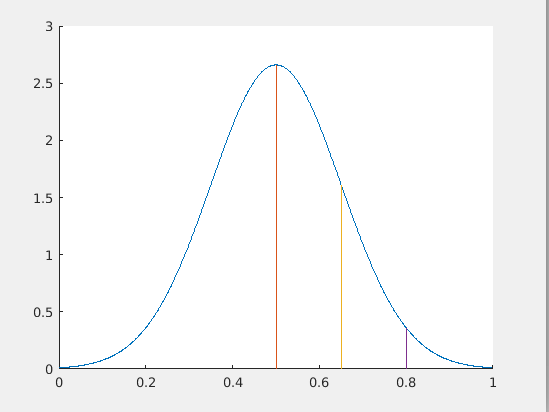
\includegraphics[scale=1]{lecture1_fig1.png}
		
		\newpage
		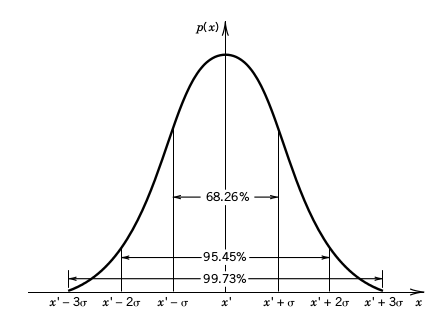
\includegraphics[scale=1.5]{lecture1_fig4.png}

		\newpage
		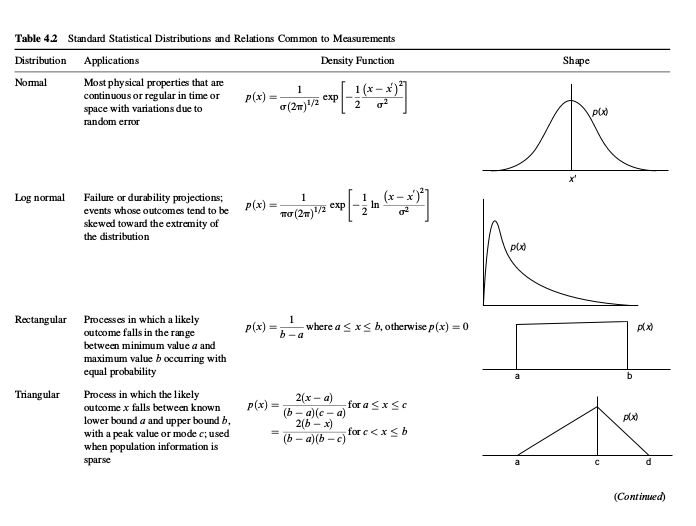
\includegraphics[scale=.8]{lecture1_fig2.png}

		\newpage
		\newpage
		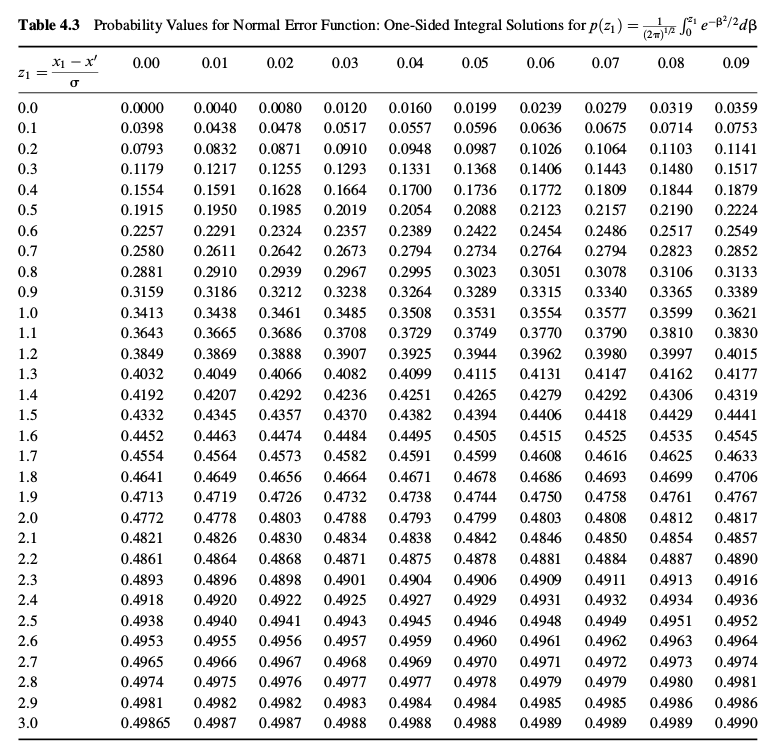
\includegraphics[scale=.8]{lecture1_fig3.png}

\end{itemize}

\end{itemize}

	

\end{document}



